\subsection{Bubblesort}
Bubble sort is a simple sorting algorithm for sorting arrays. The algorithm consists of two nested loops. The outer loop traverses the array and the inner loop traverses the part of the array starting from the current position of the outer loop. The inner loop is the workhorse here which swaps the elements if they are in the wrong order. The worst case for the algorithm occurs when the array to be sorted is actually sorted in the reverse order.

One important question about sorting is measuring the accuracy of sorting. Checking if an array is sorted is a binary question with true or false answer. Therefore in order to evaluate an approximate algorithm we need to define a measure of degree of sortedness of an array. We use the number of inversion remaining after running the approximate algorithm as a measure of sortedness. For example, if an array had 250000 inversions before sorting and it has 2500 inversions after the approximate sorting algorithm ends then the output is said to 99\% accuracy since it resolved 99\% of the inversions.

The approximation used for this algorithm is loop perforation. We tried perforating both loops at the time. The knob in this approximation is the amount of loop iterations skipped. The most aggressive setting skips every other iteration and less aggressive setting skip every 3rd, 4th, 5th, .. iteration. Perforating the inner loop consistently resulted in very poor accuracy (~50\% even with 1 in 1000 skipped iterations). Perforating the outer loop of the algorithm gave better results. In order to make sure that the sorting result are not limited to a specific input, 1000 random integer arrays of size 1000 were generated. The knob is varied from skipping every other iteration to skipping every 10th iteration. The results are shown in Table \ref{bubblesortT}. WCET is shown as a percentage of time of exact sorting and the knob value indicates the percentage of loop iterations skipped. (skipping every other iteration corresponds to 50\% and skipping every 10 iteration corresponds to 10\%). The table also shows the standard deviation in accuracy for each knob value.

\begin{table}[]
  \centering
  \caption{Bubblesort Results}
  \label{bubblesortT}
  \begin{tabular}{|l|l|l|l|}
    \hline
    \textbf{Skipped Iterations} & \textbf{Accuracy}  & \textbf{Standard Dev.}  & \textbf{WCET}           \\ \hline
50.00\% &  61.52\% &1.02\% &50.02\%   \\ \hline
33.33\% &  75.83\% &1.01\% &66.72\%   \\ \hline
25.00\% &  82.41\% &0.94\% &75.11\%   \\ \hline
20.00\% &  86.20\% &0.88\% &80.12\%   \\ \hline
16.67\% &  88.67\% &0.82\% &83.32\%   \\ \hline
14.29\% &  90.40\% &0.77\% &92.93\%   \\ \hline
12.50\% &  91.68\% &0.73\% &87.51\%   \\ \hline
11.11\% &  92.67\% &0.70\% &88.92\%   \\ \hline
10.00\% &  93.45\% &0.66\% &90.02\%   \\ \hline
  \end{tabular}
\end{table}


The results show the following with respect to our questions:

\begin{figure}
  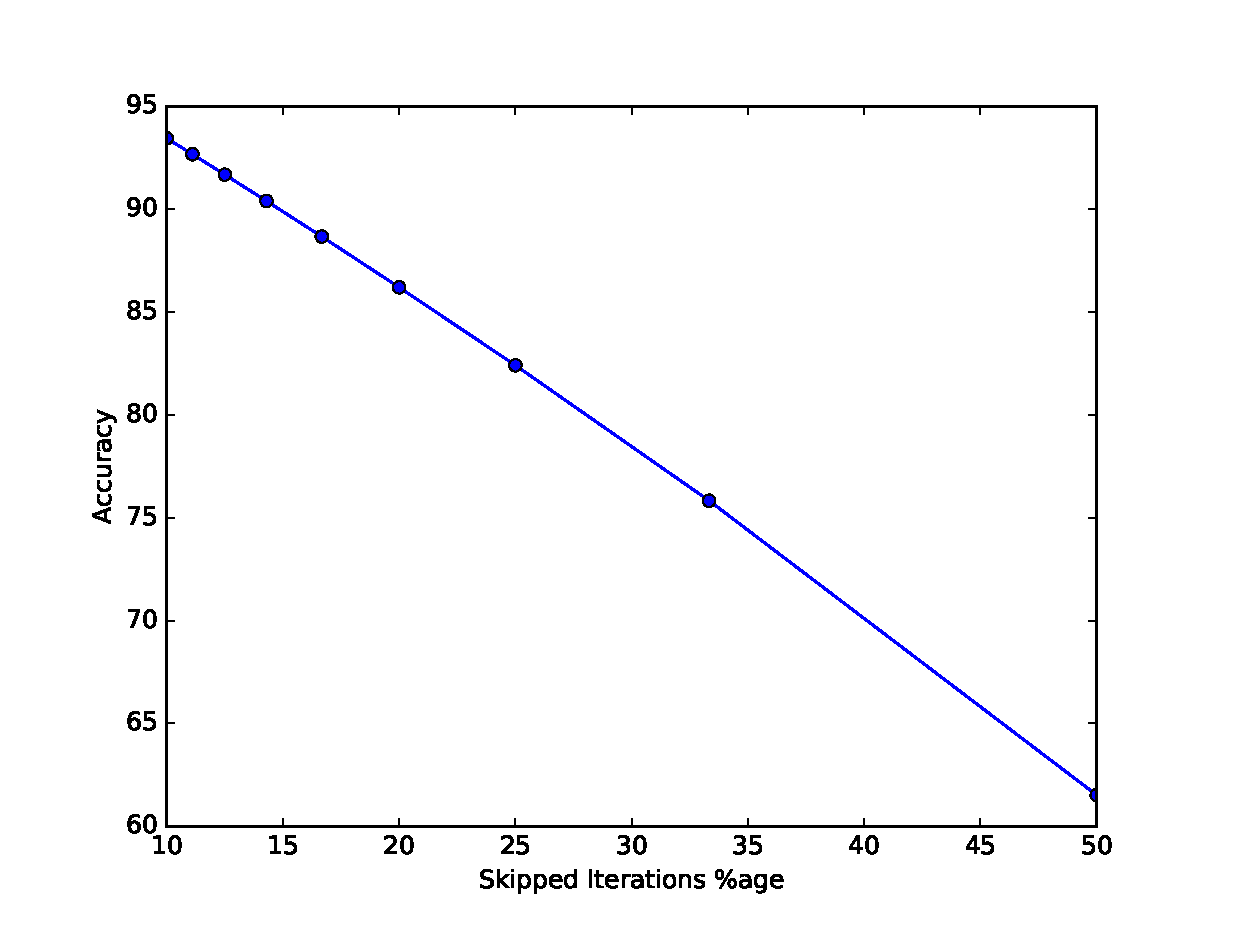
\includegraphics[width=0.95\linewidth]{Results/bubblesort1.eps}
  \caption{Accuracy vs Skipped Iterations}
  \label{bubblesort1}
\end{figure}

\begin{figure}
  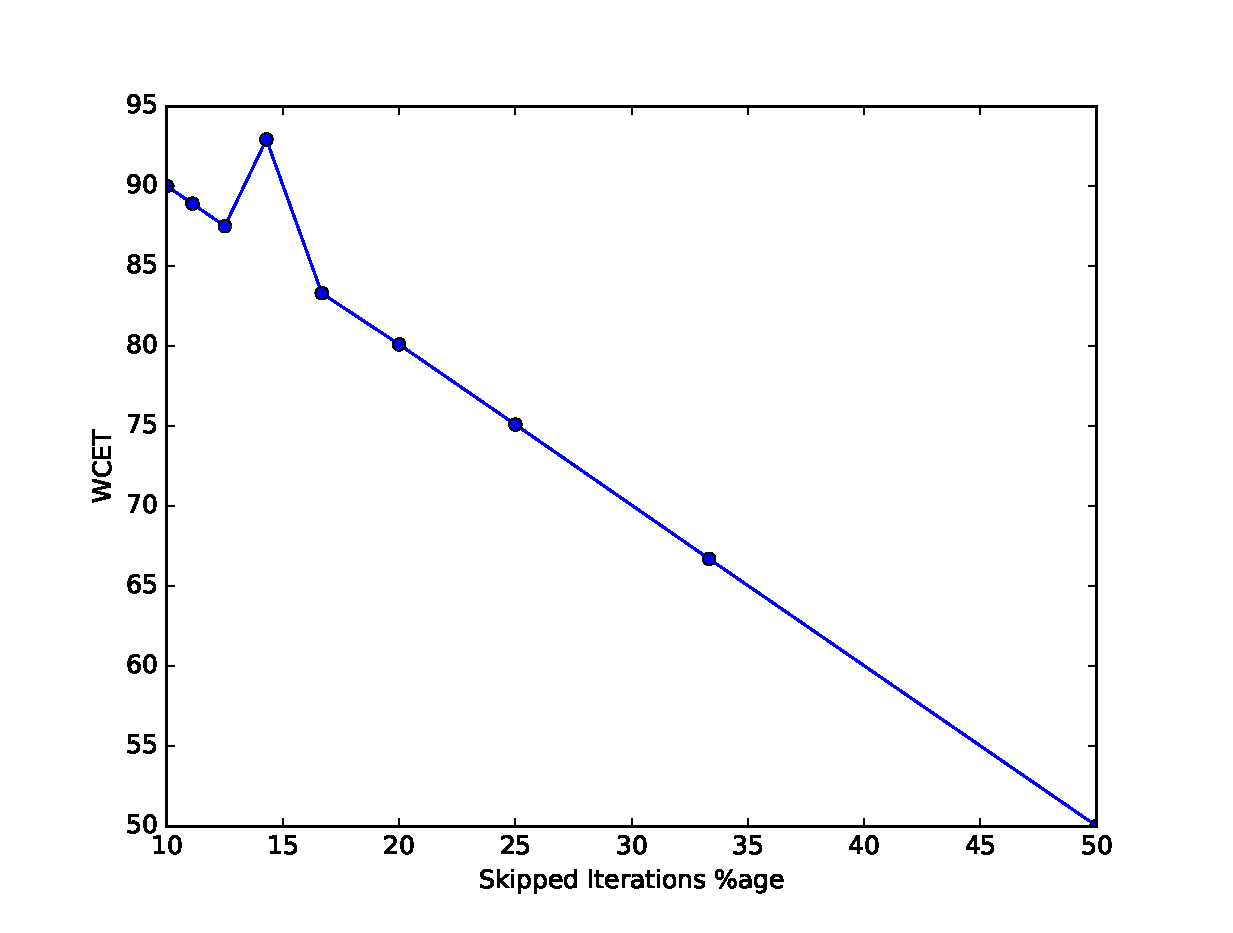
\includegraphics[width=0.95\linewidth]{Results/bubblesort2.eps}
  \caption{WCET vs Skipped Iterations)}
  \label{bubblesort2}
\end{figure}

\begin{enumerate}
\item The relation between accuracy and the number of skipped iterations is almost linear with negative slope. Accuracy is high when fewer loops are skipped. This is shown in figure \ref{bubblesort1} 
\item The relation between WCET and number of loops skipped is almost linear. The exception to the rule is the the point where every 7th iteration is skipped. The conjecture here is that the mod 7 computation somehow takes more time then the other mod computations. This anomaly is clearly visible in figure \ref{bubblesort2}.
  \item The first two relations being linear means that the last relation is also linear. This makes a good case for not using this approximation. Spending 90\% time to get 90\% accuracy is not good enough.
\end{enumerate}


%% \begin{figure}
%%   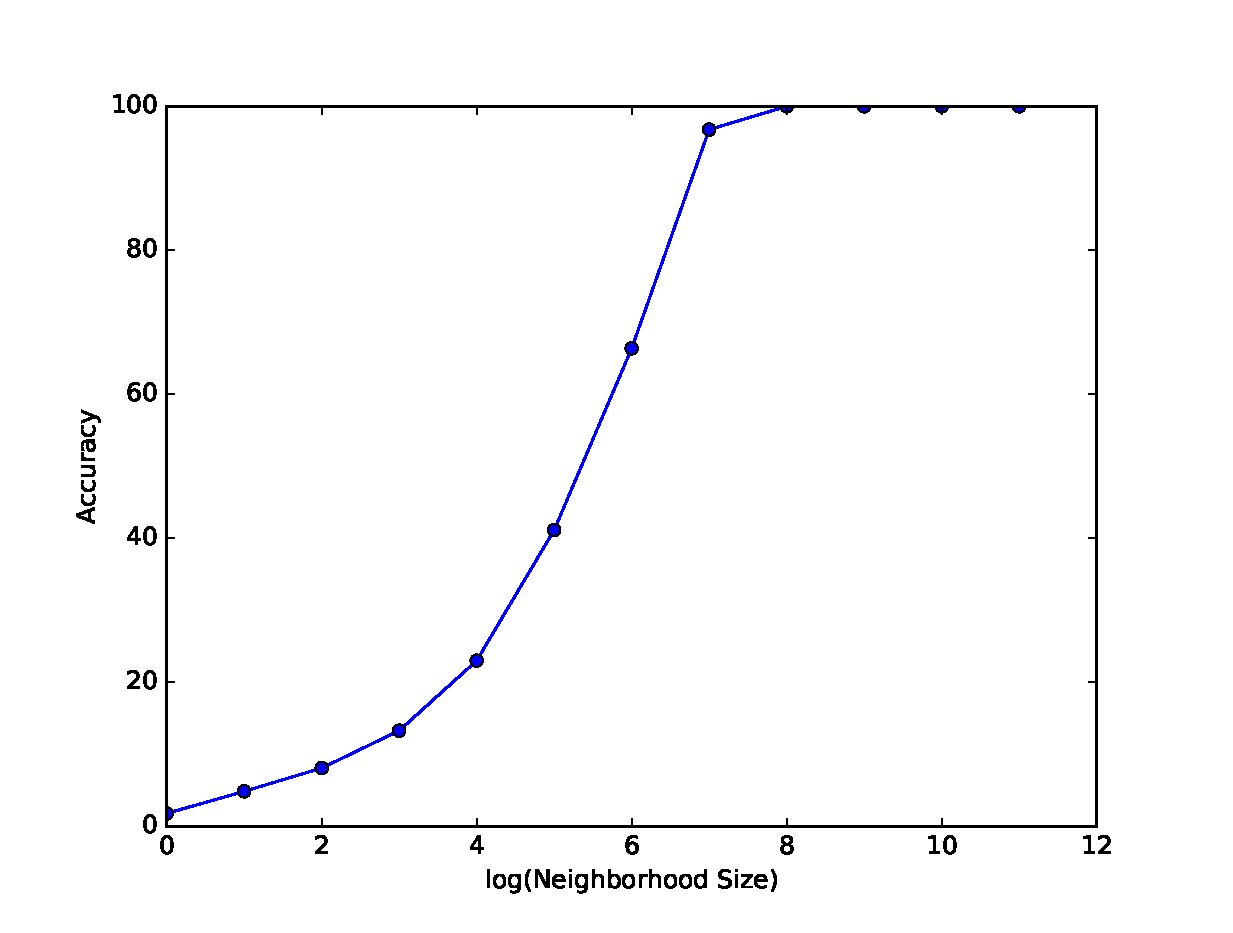
\includegraphics[width=0.95\linewidth]{Results/binarysearch1.eps}
%%   \caption{WCET vs Accuracy}
%%   \label{binarysearch3}
%% \end{figure}



